
\documentclass{article}

\usepackage[utf8]{inputenc}
\usepackage[fontsize=5.5pt]{scrextend}
\usepackage{thmbox}
\usepackage{multicol}
\setlength{\parindent}{1pt}
\usepackage{amsmath, amssymb, amsthm}
\usepackage{booktabs, tabularx}
\usepackage{setspace}
\usepackage{geometry}
\geometry{a4paper,left=0.5cm,right=0.5cm,top=0.5cm,bottom=0.5cm}
\usepackage{wrapfig}
\usepackage{graphicx} 
\usepackage{float} 
\usepackage{subfigure}

\begin{document}


\begin{tabular}{ccccc}
\toprule  
Distribution & pdf/pmf  & E(X) & Var(X) & MGF \\
\midrule  
Binomial & $f(x \mid n,p) = {n \choose k} p^{k}(1-p)^{n-k}$ & $ np $ & $ np(1-p)$ & $(1-p+ p e^{t})^{n}$\\

\midrule  
D Unif & $f(x\mid N) = \frac{1}{N}$ & $\frac{N+1}{2}$ & $\frac{(N+1)(N-1)}{12}$ & $\frac{1}{N}\sum^{N}_{i = 1} e^{it}$ \\

\midrule  
Geometric & $f(x\mid p) = p(1-p)^{x-1}$ & $\frac{1}{p}$ & $\frac{(1-p)}{p^2}$ & $\frac{pe^t}{1-(1-p)e^t} \ t<-log(1-p)$ \\

\midrule  
Hypergeom & $f(x\mid N,M,K) = \frac{{M \choose x}{N-M \choose K-x}}{{N \choose K}}$ & $\frac{KM}{N}$ & $\frac{(KM)(N-M)(N-K)}{NN(N-1)}$ & -\\

\midrule  
NBinom & $f(x\mid r,p) = {r+x-1 \choose x}p^{r}(1-p)^{x}$ & $\frac{r(1 - p)}{p}$ & $\frac{r(1-p)}{p^2}$ & $(\frac{p}{1-(1-p)e^t})^r \ t<-log(1-p)$ \\

\midrule  
Poisson & $f(x\mid \lambda) = \frac{e^{-\lambda}\lambda^{x}}{x!} \ 0 \le \lambda < \infty$  & $\lambda$ & $\lambda$ & $e^{\lambda(e^{t}-1)}$ \\

\midrule  
Beta & $f(x\mid \alpha, \beta) = \frac{x^{\alpha - 1}(1-x)^{\beta - 1}}{B(\alpha,\beta)} x \in [0,1], \alpha, \beta > 0$ & $\frac{\alpha}{\alpha + \beta}$ & 
$\frac{\alpha \beta}{(\alpha + \beta)^2 (\alpha + \beta + 1)}$ & 
$1 + \sum^{\infty}_{k=1}(\prod^{k-1}_{r=0} \frac{\alpha +r}{\alpha +\beta +r})\frac{t^k}{k!}$ \\

\midrule  
Cauchy & $f(x\mid \theta, \sigma) = \frac{1}{\pi \sigma(1+(\frac{x-\theta}{\sigma})^2)} \sigma > 0 $  & - & - & - \\

\midrule  
$\chi^2$ & $f(x\mid p) = \frac{x^{p/2 -1}e^{-x/2}}{\Gamma(p/2)2^{p/2}},x\in [0, \infty)$  & $ p $ & $2p $ & $(\frac{1}{1-2t})^{p/2}$ \\

\midrule  
Exponential & $f(x\mid \beta) = \frac{1}{\beta}e^{-x/\beta} x \in [0,\infty), \beta > 0 $  & $\beta$ & $\beta^2$ & $\frac{1}{1-\beta t}, t < \frac{1}{\beta}$ \\

\midrule  
F & $f(x\mid v_1, v_2) = \frac{\Gamma(\frac{v_1 +v_2}{2})}{\Gamma(\frac{v_1}{2})\Gamma(\frac{v_2}{2})}(\frac{v_1}{v_2})^{v_{1} /2}\frac{x^{(v_1 - 2)/2}}{(1+(\frac{v_1}{v_2})x)^{(v_1 + v_2)/2}}, x \in [0,\infty)$  & $\frac{v_2}{v_2 - 2} v_2 > 2$ & $2(\frac{v_2}{v_2 - 2})^2 \frac{v_1 +v_2 -2}{v_1(v_2 - 4)}, v_2 > 4$ & $e^{\lambda(e^{t}-1)}$ \\

\midrule  
Gamma & $f(x\mid \alpha, \beta) = \frac{x^{\alpha - 1}e^{-x/ \beta}}{\Gamma(\alpha)\beta^{\alpha}}, x \in [0, \infty), \alpha, \beta > 0$  & $\alpha \beta$ & $ \alpha \beta^2$ & $(\frac{1}{1-\beta t})^{\alpha}, t < \frac{1}{\beta}$ \\

\midrule  
Normal & $f(x\mid \mu, \sigma^2) = \frac{1}{\sqrt{2\pi \sigma^2}}e^{-(x-\mu)^2/(2\sigma^2)}$  & $\mu$ & $\sigma^2$ & $e^{\lambda(e^{t}-1)}$ \\

\midrule  
T & $f(x\mid v) = \frac{\Gamma(\frac{v+1}{2})}{\Gamma(\frac{v}{2})\sqrt{v\pi}(1+\frac{x^2}{v})^{(v+1)/2}}$  & $ 0, v>1 $ & $\frac{v}{v-2}, v > 2$ & $-$ \\

\midrule  
Unif & $f(x\mid a,b) = \frac{1}{b-a}$  & $\frac{a+b}{2}$ & $ \frac{(b-a)^2}{12}$ & $ \frac{e^{bt} - e^{at}}{(b-a)t}$ \\


\bottomrule
\end{tabular}



\begin{multicols*}{3}
\section{Distribution Properties}

1. $B(\alpha, \beta) = \frac{\Gamma(\alpha)\Gamma(\beta)}{\Gamma(\alpha+\beta)} = \int^1_0 x^{\alpha - 1}(1-x)^{\beta - 1} dx$ \\

2. $F_{v_1,v_2} = (\frac{\chi^2_{v_1}}{v_1})/(\frac{\chi^2_{v_2}}{v_2}), \chi^2s$  are independent 
3. $F_{1,v} = T_v^2$\\

4. $Gamma(1,\beta) = Exponential(\beta)$ \\

5. $Gamma(p/2, 2) = \chi^2_p$; $X \backsim Gamma(\alpha, \beta), Y \backsim Poisson(X/\beta)$ then $P(X\le x) = P(Y \ge \alpha)$ \\

6. $X_1,...,X_n \backsim Poisson(\lambda) $  Then $\sum X_i \backsim Poisson(n\lambda)$ \\

7. $X_1,.,X_{\alpha} \backsim Exponential(\beta)$, then $\sum x_i \backsim Gamma(\alpha,\beta), \Bar{X} \backsim Gamma(\alpha, \beta/\alpha)$ \\
8. $X \backsim Gamma(\alpha, \beta), P(X \le x) = P(Y \ge \alpha), Y \backsim Poisson(x/\beta) $ \\
9. $ Z \backsim N(0,1), Z^2 \backsim \chi^2_{1}$\\
10. $ X_i \backsim \chi^2_{p_I}$ then $\sum X_i \backsim \chi^2_{\sum p_i}$\\
11. $T = \frac{U}{\sqrt{V/p}} = \frac{\Bar{X} - \mu}{S/\sqrt{n}}, U \backsim N(0,1), V \backsim \chi^2_p$\\
12. $X  \backsim Binomial(n, p), Y \backsim Beta(x, n-x+1)$ then $P(X \ge x )= P(Y \le p)$\\
13. $X_1, .., X_n \backsim Unif(0,1)$ (can use F(X) to get uniform) then asymptotically $nU_{(1)} \to Exp(1), n(1-X_{(n)}) \to Exp(1)$ \\
14. $F = (S^2_X / \sigma^2_X)/(S^2_Y / \sigma^2_Y) \backsim F_{n-1,m-1}$\\
$(n-1)S^2/\sigma^2 \backsim \chi^2_{n-1}, X_1,..,X_n\backsim N(\mu,\sigma^2)$,\\ $S^2 = \sum(X_i - \Bar{X})/(n-1)$\\
15. $X \backsim T_q, X^2 \backsim F_{1, q}$; $Y \backsim F_{p,q}, (p/q)Y/(1 + (p/q)Y) \backsim Beta(p/2, q/2)$

\begin{thmbox}{Gamma Function}
$\Gamma(\alpha) = \int^{\infty}_{0}t^{\alpha - 1}e^{-t}dt$
\begin{enumerate}
\item [1.]$\Gamma(\alpha + 1) = \alpha\Gamma(\alpha)$
\item [2.] $\Gamma(n) = (n-1)!$
\item [3.] $\Gamma(\frac{1}{2}) = \sqrt{\pi}$
\item [4.] $\Gamma(1) = 1$
\item[5.] $\int^{\infty}_{0} t^{\alpha - 1} e^{-\beta t} dt = \Gamma(\alpha)(\frac{1}{\beta})^{\alpha}$
\end{enumerate}
\end{thmbox}

\begin{thmbox}{Bivariate Normal}
Bivariate N(X,Y) with $\mu_x,\mu_y,\sigma^2_x, \sigma^2_y, \rho , Z_1,Z_2 iid N(0,1)$\\
$X = \sigma_{x}Z_1 + \mu_x$\\
$Y = \sigma_y(\rho Z_1 + \sqrt{1-\rho^2}Z_2)+\mu_y$ \\
$aX + bY \backsim N(a\mu_x +b\mu_y, a^2\sigma^2_x + b^2\sigma_y^2 + 2ab\rho\sigma_x\sigma_y)$
\end{thmbox}

\begin{thmbox}{Normal Sum}
$X \backsim N(\mu, \sigma^2), Y \backsim N(\gamma, \tau^2), X,Y $ are independent, then
$Z = X + Y \backsim N(\mu + \gamma, \sigma^2 + \tau^2)$
\end{thmbox}

\begin{thmbox}{Exponential Family}

$f(x\mid \theta) = h(x)c(\theta)exp(\sum^{k}_{i=1}w_i(\theta)t_i(x))$
\end{thmbox}

\begin{thmbox}{Stein's Lemma}
$X \backsim N(\theta,\sigma^2)$ and $g$ is a differentiable function satisfying $E\arrowvert g'(x)\arrowvert < \infty$ \\ 
then $E[g(x)(x-\theta)] = \sigma^2E(g'(x))$
\end{thmbox}

\begin{thmbox}{Multinomial Theorem}
$ A = \{(x_1,..,x_n):\sum^{n}_{i=1}x_i = m\}$\\
$(p_1 + ..+p_n)^n = \sum_{x \in A} \frac{m!}{x_1!...x_n!}p_1^{x_1}....p_n^{x_n}$
\end{thmbox}

\begin{thmbox}{Location-Scale Family}
    $-\infty < \mu < \infty, \sigma > 0, z \backsim f(z)$, the location- scale family indexed by $\mu, \sigma$ is $X = \sigma Z + \mu , X \backsim \frac{1}{\sigma}f((x - \mu)/\sigma)$
\end{thmbox}


\section{Calculation}
\subsection{e related}
$e^x = \sum^{\infty}_{n = 0}\frac{x^n}{n!}$\\
$e^a =  \lim_{n \to \infty}(1+\frac{a}{n})^n$


\subsection{Sum related}
$S_n = \frac{a_1(1-q^n)}{1-q}$\\
$\sum^{\infty}_{i =1}\frac{1}{i^2} = \frac{\pi^2}{6}$\\
$\sum^{n}_{k = 1}k^2 = \frac{n(n+1)(2n+1)}{6}$\\
$\sum^{n}_{i = 1}(x_i - a)^2 = \sum^{n}_{i = 1}(x_i - \Bar{x})^2 + \sum^{n}_{i =1}(\Bar{x} - a)^2$\\
$ \sum^{n}_{i = 1}(x_i - \Bar{x})^2 = \sum^{n}_{i = 1}x_i^2 - n\Bar{x}^2$\\
$\min\sum(x_i -a)^2 = \sum(x_i - \Bar{x})^2$

\subsection{Integral and Series}
$ \int^{\infty}_{-\infty}e^{-ax^2+bx+c}dx = \sqrt{\frac{\pi}{a}}e^{\frac{b^2}{4a}+c}$\\
$\int uv'dx = uv - \int u'vdx$\\
$ f(x) = \sum^{\infty}_{n=0}\frac{f^{n}(x_0)}{n!}(x-x_0)^n$\\
$\int^{1}_{0}p^{t}(1-p)^{k-t}dp = \frac{t!(k-t)!}{(k+1)!}$\\
$ \int^{\infty}_{0}e^{-\frac{x^2}{2}}dx = \sqrt{\frac{\pi}{2}}$\\
$ n! \approx \sqrt{2\pi n}(\frac{n}{e})^n$\\
\begin{thmbox}{Leibnitz's Rule}
If $f(x,\theta)$ and $a(\theta), b(\theta)$ are differentiable with respect to $\theta$, then\\
$\frac{d}{d\theta}\int^{b(\theta)}_{a(\theta)}f(x,\theta)dx = f(b(\theta),\theta)\frac{d}{d\theta}b(\theta) - \\f(a(\theta),\theta)\frac{d}{d\theta}a(\theta) +
\int^{b(\theta)}_{a(\theta)}\frac{\partial}{\partial\theta}f(x,\theta)dx$
\end{thmbox}
\subsection{Inequality}

\begin{thmbox}{Bonferroni's Inequality}
$P(A \bigcap B) \ge P(A) + P(B) - 1 $
\end{thmbox}

\begin{thmbox}{Chebychev's Inequality}
Let $X$ be a random variable and let $g(x)$ be a nonnegative function, then for any \\
$r > 0, P(g(X)\ge r) \le \frac{E(g(X))}{r}$
\end{thmbox}

\begin{thmbox}{Holder's Inequality}
$\frac{1}{p} + \frac{1}{q} = 1$ then
$\frac{1}{p}a^p +\frac{1}{q}b^q \ge ab$, $a,b,p,q > 0$ \\
$\lvert E(XY) \rvert \le E\lvert XY \rvert \le (E\lvert X\rvert ^p)^{1/p}(E\lvert  Y\rvert ^q)^{1/q}$
\end{thmbox}

\begin{thmbox}{Jensen's Inequality }
 $g(x)$ is convex, then 
$Eg(X) \ge g(EX)$
\end{thmbox}

\begin{thmbox}{Convex Function}
A function $g(x)$ is convex if $g(\lambda x + (1 - \lambda)y) \le \lambda g(x) + (1 - \lambda)g(y)$ for all $x$ and $y$, and $0 < \lambda < 1$. \\
Or $g''(x) \ge 0$
\end{thmbox}

\section{Probability}
\begin{tabular}{ccc}
\toprule  
 & Without replace & with replace \\
\midrule
Ordered & $\frac{n!}{(n-r)!}$ & $n^r$ \\
Unordered & ${n \choose r} $ & $ {n+r-1 \choose r}$\\
\bottomrule
\end{tabular}


\subsection{Transformation}
\begin{thmbox}{Univariate Transformation}
1. $Y = g(X), g(x)$ is a monotone function \\
2. $f_X(x)$ is continuous on X \\
3. $g^{-1}(y)$has a continuous derivative on y \\
Then $f_Y(y) = f_X(g^{-1}(y))\lvert \frac{d}{dy}g^{-1}(y)\rvert, y \in y$
\end{thmbox}

\begin{thmbox}{Univariate Transformation with non-monotone}
\begin{enumerate}
\item [1.]Partition $A_0,A_1,......,A_k$ of $x$
\item [2.]there exist $g_i(x)$ satisfies, $g_i(x)$ is monotone on $A_i$ and $g^{-1}(y)$ has a continuous derivative on $y$
\end{enumerate}
Then $f_Y(y) = \sum^{k}_{i=1}f_X(g_{i}^{-1}(y))\lvert \frac{d}{dy}g_{i}^{-1}(y)\rvert, y \in y$
\end{thmbox}

\begin{thmbox}{Bivariate Transformation}
$A = \{(x,y): f_{X,Y}(x,y) > 0\}, \\ B = \{(u,v): u = g_1(x,y), v = g_2(x,y)\}$ \\ assume one-to-one and $x = h_1(u,v), y = h_2(u,v)$\\
 
\begin{equation}
J =
\begin{vmatrix}
\frac{\partial x}{\partial u} & \frac{\partial x}{\partial v}\\
\frac{\partial y}{\partial u} & \frac{\partial y}{\partial v}\\
\end{vmatrix} 
\end{equation}
$f_{U,V}(u,v) = f_{X,Y}(h_1(u,v), h_2(u,v))\lvert J\rvert$ \\

When not one-to-one, suppose $A_1,....,A_k$ form a partition of $A$, 
\begin{equation}
\begin{cases}
U = g_1(x,y) \\ 
V = g_2(x,y)
\end{cases}    
\end{equation}

is one-to-one from $A_i$ to $B$ then\\
$f_{U,V}(u,v) =\sum^{k}_{i=1} f_{X,Y}(h_{i,1}(u,v), h_{i,2}(u,v))\lvert J_i\rvert$
\end{thmbox}
\begin{thmbox}{Inverse Uniform}
Let $X$ have continuous cdf $F_X(x)$ and define the random variable $Y = F_X(X)$. Then $Y \thicksim Unif(0,1)$.
\end{thmbox}

\subsection{MGF}
$M_X(t) = E(e^{tx})$, $E(X^n) = M_X^{(n)}(0)$\\
$M_{aX + b}(t) = e^{bt}M_X(at)$
\begin{thmbox}{Sum of r.v}
$X,Y$ are independent with mgf $M_X(t), M_Y(t)$ then $Z = X + Y \rightarrow M_Z(t)  = M_X(t)M_Y(t)$
\end{thmbox}


\subsection{Hierarchical Models}
$E(X) = E(E(X\mid Y))$\\
$Var(X) = E(Var(X \mid Y)) + Var(E(X \mid Y))$

\subsection{Order Statistics}
\subsubsection{Discrete}
$P(X_{(j)}\le x_i) = \sum^{n}_{k = j}{n \choose k}P_i^k(1-P_i)^{n-k}, \\ P_i = \sum^{i}_{j =1}p_j$ \\

\subsubsection{Continuous}
$ F_{(X_{(j)})}(x) = \sum^{n}_{k = j}{n \choose k} [F_{X}(x)]^k[1-F_{X}(X)]^{n-k}$\\
$f_{X_{(j)}}(x) = \frac{n!}{(j-1)!(n-j)!}f_X(x)[F_X(x)]^{j-1}[1-F_X(x)]^{n-j}$ \\
\begin{equation}
\begin{aligned}
f_{X_{i}, X_{j}}(u,v) = \left( \frac{n!}{(i-1)!(j-i-1)!(n-j)!}f_X(u)f_X(v) \right. \\
\left. [F_X(u)]^{i-1}[F_X(v) - F_X(u)]^{j-i-1}[1-F_X(v)]^{n-j} \right)
\end{aligned}
\end{equation} \\

\subsection{Convergence}

\begin{thmbox}{Convergence}
1. In Probability: $\lim_{n \to \infty} P(\lvert X_n - X\rvert \le \epsilon) = 1$ \\
2. Almost Sure: $P(\lim_{n \to \infty} \lvert X_n - X\rvert \le \epsilon) = 1$ \\
3. Distribution: $\lim_{n \to \infty} F_{X_n}(x) = F_X(x)$, at all $x, F_X(x)$ is continuous.
\end{thmbox}
\begin{thmbox}{Slutsky's Theorem}
If $X_n \rightarrow X$ in distribution and , $Y_n \rightarrow a $ in probability, a is a constant, then \\
$Y_n X_n \rightarrow aX $ in distribution \\
$X_n +Y_n \rightarrow X + a$ in distribution
\end{thmbox}

\begin{thmbox}{First Order Taylor Approximation}
r.v.s $T_1, ..,T_k$ have means $\theta_1,...,\theta_k$ and $\boldsymbol{T} = (T_1,..,T_k), \boldsymbol{\theta} = (\theta_1, .., \theta_k)$. Define $g'_i(\boldsymbol{\theta}) = \frac{\partial}{\partial t_i}g(\boldsymbol{t})\mid_{t_1 = \theta_1,....,t_k=\theta_k}$\\
$E_{\theta}(g(\boldsymbol{T})) \approx g(\boldsymbol{\theta}) + \sum^{k}_{i = 1}g'_i(\theta)E_{\theta}(T_i - \theta_i) = g(\boldsymbol{\theta})$\\
$Var(g(\boldsymbol{T})) \approx \sum^{k}_{i = 1} [g'_i(\boldsymbol{\theta})]^2 Var(T_i) + 
2\sum_{i > j}g'_i(\boldsymbol{\theta})g'_j(\boldsymbol{\theta})Cov(T_i, T_j)$
\end{thmbox}
\clearpage
\begin{thmbox}{Delta Method}
\textbf{First Order:} Let $Y_n$ be a sequence of r.v.s that satisfies $\sqrt{n}(Y_n - \theta) \rightarrow N(0,\sigma^2)$ in distribution. For a given function $g$ and a specific value of $\theta$, suppose that $g'(x)$ exists and is not $\theta$, then \\
$\sqrt{n}(g(Y_n) - g(\theta)) \rightarrow N(0, \sigma^2(g'(\theta))^2)$\\
\textbf{Second Order:} suppose $g'(\theta) = 0$ and $g''(\theta)$ exists and is not 0, then \\
$n[g(Y_n) - g(\theta)] \rightarrow \sigma^2\frac{g''(\theta)}{2}\chi^2_1$ in distribution.\\
\textbf{Multivariate:} $X_1, ..., X_n, E(X_{ij}) = \mu_i,\\ Cov(X_{ik}, X_{jk}) = \theta_{ij}, \tau^2 = \sum \sum \theta_{ij}\frac{\partial g(\mu)}{\partial \mu_i }\frac{\partial g(\mu)}{\parital \mu_j} \\ 
\sqrt{n}[g(\Bar{X_1},..,\Bar{X_s}) - g(\mu_1,..,\mu_p)]\to^{D} N(0,\tau^2) $ \\
\textbf{General:} if $g'(a)$ exists and $n^b(X_n - a) \to^D X$ for $b > 0$, then $n^b(g(X_n) - g(a)) \to^D g'(a)X$
\end{thmbox}


\section{Data Reduction}

\begin{thmbox}{Sufficient  Stat}
if $\frac{f_X(x\mid \theta)}{f_{T(X)}(T\mid\theta)}$ is constant as a function of $\theta$, $T(X)$ is a sufficient statistic for $\theta$.
\end{thmbox}

\begin{thmbox}{Factorization}
Let $f(x|\theta)$ be a joint pmf or pdf of sample $X$. A statistic $T(x)$ is sufficient for $\theta$ iff $\exists g(t|\theta), h(x)$ s.th $\forall x,\theta$ $f(x|\theta) = g(T(x)|\theta)h(x)$
\end{thmbox}



\begin{thmbox}{Exponential Sufficiency}
Let $X_1,\dots,X_n$ iid observations from pdf or pmf $f(x|\theta)$ that belongs to the exponential family given by

$$
f(x|\theta) = h(x)c(\theta)\exp\left[\sum_i^kw_i(\theta)t_i(x)\right]
$$

Them, for $\theta = (\theta_1,\dots,\theta_d), d\leq k$

$$
T(X) = \left(\sum_j^n t_1(x_j),\dots,\sum_j^nt_k(x_j)\right)
$$
Is sufficient for $\theta$.
\end{thmbox}

\begin{thmbox}{Minimal Sufficient Statistic}
Let $f(x\mid \theta)$ be the pdf or pmf of sample $X$. Suppose $\exists T(X)$ s.th. $\forall X,Y\in\mathcal{X}$ the ratio $f(X|\theta)/f(Y|\theta)$ is a constant function of $\theta$ iff $T(X) = T(Y)$. Then $T$ is minimal.
\end{thmbox}

\begin{thmbox}{Basu's Theorem}
\textbf{1.}If $T(X)$ is complete and minimal suficient statistic, then $T(X)$ is independent from all ancicially statiscs. \\
\textbf{2.}If minimal suffucient statistic exists, then any complete statistic is also a minimal sufficient statistic.
\end{thmbox}

\begin{thmbox}{Complete stat. in the expo family} Same set up as Thm 6.2.10, then $T(X)$ is a complete statistic if $\{(w_1(\theta),\dots,w_k(\theta)):\theta\in\Theta\}$ contains an open set in $\mathbb{R}^k$.

A counter example: $N(\theta,\theta^2)$.
\end{thmbox}

\begin{thmbox}{Complete Statistic}
Let $f(x\mid \theta)$ be a family of pdfs or pmfs for a statistic $T(X)$. The family of probability distributions is called complete if $E_\theta g(T) = 0$ for all $\theta$ implies $P_\theta(g(T) = 0) = 1$ for all $\theta$. Equivalently, $T(X)$ is called complete statistic.
\end{thmbox}

\begin{thmbox}{Ancillary Statistic}
A statistic $S(X)$ is an ancillary statistic if its distribution does not depend on the parameter.
\end{thmbox}


\section{Point Estimation}

\begin{thmbox}{Newton Method}
    1-D: iterate $\theta^{(t + 1)} = \theta^{(t)} - l'(\theta^{(t)}) / l''(\theta^{(t)})$\\
    2-D: iterate $\theta^{(t + 1)} = \theta^{(t)} - l''(\theta^{(t)})^{-1}l'(\theta^{(t)}) $ where $l''(\theta^{(t)})^{-1}$ is the matrix inverse
\end{thmbox}
\begin{thmbox}{Two Dimension Optimization}
    Verify a function $H(\theta_1, \theta_2)$ has a local maximum: \\
    1. first order partial derivative are 0\\
    2. at least one second order partial derivative derivative is negative \\
    3. Hessian Matrix is positive\\
    
\end{thmbox}
\begin{thmbox}{Mean Squared Error}
$E_{\theta}(W-\theta)^2 = Var_{\theta}W +(Bias_{\theta}W)^2$\\
$Bias_{\theta}W = E_{\theta}(W) - \theta$
\end{thmbox}

\begin{thmbox}{Invariance MLE}
If $\hat\theta$ is the MLE of $\theta$, then $\forall \tau(\theta)$, the MLE of $\tau(\theta)$ is $\tau(\hat\theta)$.
\end{thmbox}

\begin{thmbox}{Best Unbiased Estimator}
An estimator $W^*$ is best unbiased estimator of $\tau(\theta)$ if it satisfies $E_\theta W^* = \tau(\theta),\forall\theta$, and for any $W\in \{W:E_\theta W(X) = \tau(\theta), \forall \theta\}$ $Var_\theta(W^*) < Var_\theta(W)\forall \theta$ . This is also called uniform minimum variance unbiased estimator (UMVUE) of $\tau(\theta)$.

\end{thmbox}

\begin{thmbox}{Cramer-Rao Inequality}
Let $X_1,\dots, X_n$ be a sample with pdf $f(x|\theta)$ , and let $W(X) = W(X_1,\dots,X_n)$ be any estimator satisfying
$$
\frac{d}{d\theta}E_{\theta}W(X) = \int_\mathcal{X}\frac{\partial}{\partial\theta}\left[W(x)f(x|\theta)\right]dx,\text{ and}
$$

$Var_\theta(W(X)) <\infty$, then 

$$
Var_\theta(W(X)) \geq \frac{\left(\frac{d}{d\theta}E_\theta W(X)\right)^2}{E_\theta\left(\left(\frac{\partial}{\partial}\log f(x|\theta)\right)^2\right)}
$$

NOTE: The Cramer-Rao theorem does not apply to cases in which the range of the pdf depends on the parameter!!!! Which implies we don't know what is the actual lower bound!!!
\end{thmbox}



\begin{thmbox}{Cramer-Rao Inequality iid case}
If the assumptions of theorem 7.3.9 are satisfied, and, additionally if the sample is iid with pdf $f(x_i|\theta)$, then
$$
Var_\theta(W(X)) \geq \frac{\left(\frac{d}{d\theta}E_\theta W(X)\right)^2}{nE_\theta\left(\left(\frac{\partial}{\partial\theta}\log f(x_i|\theta)\right)^2\right)}
$$

\end{thmbox}

\begin{thmbox}{Fisher Information}
Fisher Information = $E_{\theta}((\frac{\partial}{\partial \theta}log L(x\mid \theta))^2)$\\

If $f(x_i|\theta)$ satifies

\begin{multline}
\frac{d}{d\theta}E_\theta\left(\frac{\partial}{\partial\theta}\log f(X|\theta)\right) = \\%
\int\frac{\partial}{\partial\theta}\left[ 
\left(\frac{\partial}{\partial\theta}\log f(x|\theta)\right)% 
f(x|\theta)\right]dx
\end{multline}
Which is true for exponential families, then

$$
E_\theta\left(\left(\frac{\partial}{\partial}\log f(x_i|\theta)\right)^2\right) = - E_\theta\left(\frac{\partial^2}{\partial\theta^2}\log f(x_i|\theta)\right)
$$

\end{thmbox}

\begin{thmbox}{Attainment}
Let $X_1,\dots,X_n$ be iid $f(x|\theta)$ where the pdf satisfies the conditions of the Cram\'er-Rao theorem. Let the joint likelihood function be $L(\theta|X)$. If $W(X)$ is any unbiased estimator of $\tau(\theta)$, then $W(X)$ attains the Cram\'er-Rao lowerbound iff

$$
a(\theta)\left[W(X) - \tau(\theta)\right] = \frac{\partial}{\partial\theta}\log L(\theta|X)
$$
For some function $a(\theta)$.

\end{thmbox}

\begin{thmbox}{Rao-Blackwell}
Let $W$ be any unbiased estimator of $\tau(\theta)$, and let $T$ be a sufficient statistic for $\theta$. Define $\phi(\theta) = E(W|T)$. Then $E_\theta\phi(T) = \tau(\theta)$, and $Var_\theta\phi(T)\leq Var_\theta(W)$ for all $\theta$ (so the new is uniformly better unbiased than the previous).
\end{thmbox}

\begin{thmbox}{Uniqueness of UMVUE}
If $W$ is best unbiased estimator of $\tau(\theta)$, then $W$ is unique.
\end{thmbox}

\begin{thmbox}{if adding noise improves, then it is a bad estimator}
If $E_\theta(W)=\tau(\theta)$, $W$ is the best unbiased estimator of $\tau(\theta)$ $\iff$ $Cor(W,W') = 0$ for all $W'$ unbiased estimators of 0. 
\end{thmbox}

\begin{thmbox}{Use suff and complete to find UMVUE}
Let $T$ be a complete sufficient statistic for a parameter $\theta$, and let $\phi(T)$ be any estimator based only on $T$. Then $\phi(T)$ is the unique best unbiased estimator of its expected value
\end{thmbox}


\begin{thmbox}{Lehmann-Scheff\'e}
Unbiased estimators based on complete sufficient statistics are unique.
\end{thmbox}


\section{Hypothesis Test}

\begin{tabular}{lcc}
\toprule Truth & Accept & Reject \\ \midrule
$H_0$ & correct & Type I\\
$H_1$ & Type II & correct \\ \bottomrule
\end{tabular}



\begin{thmbox}{Definition on tests}

{\bf Power function} $\beta(\theta) = \Pr_{\theta}(X\in R)$

{\bf $\alpha$-level(size)} $\sup_{\theta\in\Theta_0}\beta(\theta) \leq(=) \alpha$

{\bf Unbiased} $\beta$ is unbiased if $\forall\{\theta'\in \Theta_0^c, \theta''\in\Theta_0\},\, \beta(\theta') \geq \beta(\theta'')$

{\bf p-value} $p(X) = \sup_{\theta \in \theta_0}P_{\theta}(W(X) \ge W(x))$ 
\end{thmbox}

\begin{thmbox}{UMP Test}
Let $\mathcal{C}$ be the class of test for testing $H_0:\theta\in\Theta_0$ vs $H_1:\theta\in\Theta_0^c$. A test in class $\mathcal{C}$, with power function $\beta(\theta)$, is a {\it uniformly most powerful} (UMP) {\it class $\mathcal{C}$ test} if $\beta(\theta) \geq \beta'(\theta)$ for every $\theta\in\Theta_0^c$ and every $\beta'(\theta)$ that is a power function of a test in class $\mathcal{C}$.
\end{thmbox}

\begin{thmbox}{Neyman-Pearson Lemma}
Consider testing $H_0:\theta=\theta_0$ vs $H_1:\theta=\theta_1$, where the corresponding to $\theta_i$ is $f(x|\theta_i)$, $i=0,1$, using a test with rejection region $R$ that satisfies
\begin{equation}
\tag{8.3.1}
\begin{aligned}
&x\in R\mbox{ if }f(x|\theta_1) > kf(x|\theta_0), \mbox{ and} \\
&x\in R^c\mbox{ if }f(x|\theta_1) < kf(x|\theta_0)
\end{aligned}
\end{equation}
for some $k\geq 0$,and

\begin{equation}
\tag{8.3.2}
\alpha = \Pr_{\theta_0}(X\in R)
\end{equation}
Then
\begin{enumerate}
\item (Sufficiency) Any test that satisfies both is a UMP level $\alpha$ test.
\item (Necessity) If such test exists with $k>0$, then every UMP level $\alpha$ test is a size $\alpha$ test and every UMP level $\alpha$ test satisfies (8.3.1) except perhaps on a set $A$ satisfying $\Pr_{\theta_0}(X\in A) = \Pr_{\theta_1}(X\in A)=0$.
\end{enumerate}

\end{thmbox}

\begin{thmbox}{Sufficient and NP lemma}
If $T\sim g(t \mid \theta)$ is a sufficient estimator of $\theta$, then the UMP can be built using  $g(t \mid \theta)$ instead.
\end{thmbox}

\begin{thmbox}{MLR}
$\theta_2 > \theta_1, \frac{g(t \mid \theta_2)}{ g(t \mid \theta_1)}$ is a monotone function of $t$ on $\{t:g(t\mid \theta_1) > 0 \  or \ g(t\mid \theta_2) > 0\}$
\end{thmbox}
\begin{thmbox}{Karlin-Rubin}
For $H_0: \theta\leq\theta_0$ vs $H_1: \theta>\theta_0$. For $T$ sufficient for $\theta$, if $g(t|\theta)$ has the Monotone Likelihood Ratio property, then $\forall t_0$ for which the test rejects if $T>t_0$ is a UMP  level $\alpha$ test, where $\alpha = P_{\theta_0}(T > t_0)$. \\
For $H_0: \theta\geq\theta_0$ vs $H_1:\theta<\theta_0$. $T < t_0$ is a UMP level $\alpha = P_{\theta_0}(T<t_0)$ test.
\end{thmbox}

\section{Interval Estimation}

\begin{thmbox}{Concept of CI}
   1. Coverage Probability: $P(\theta \in [L(X), U(X)]\lvert \theta)$ \\ 
   2. Confidence Coefficient: $\inf_{\theta}P(\theta \in [L(X), U(X)])$
\end{thmbox}

\begin{thmbox}{Location-Scale Pivote}
    \begin{tabular}{cc}
        \toprule  
        pdf & pivote \\
        \midrule  
        $f(x-\mu)$ & $\Bar{X} - \mu$  \\
        \midrule
        $\frac{1}{\sigma}f(\frac{x}{\sigma})$ & $\frac{\Bar{X}}{\sigma}$ \\
        \midrule
        $\frac{1}{\sigma}f(\frac{x - \mu}{\sigma})$ & $\frac{\Bar{X}-\mu}{S}$ \\
        \bottomrule
    \end{tabular} \\
    if $f(t \lvert \theta) = g(Q(t,\theta))\lvert \frac{\partial}{\partial t} Q(t,\theta)\rvert$ then $Q(T,\theta)$ is pivote, speciall case $g = 1, Q(T,\theta) = F_{\theta}(T)$ 

\end{thmbox}

\begin{thmbox}{Pivoting a CDF}
    Let T be a statistic with cdf $F_T(t\lvert\theta), \alpha_1 + \alpha_2 = \alpha \in (0,1)$ \\
    1. If $F_T(t\lvert \theta)$ is a decreasing function of $\theta$: $P(T \le t \lvert \theta_U(t)) = \alpha_1 / F_T(t \lvert \theta_U(t)) = \alpha_1, P(T \ge t \lvert \theta_L(t)) = \alpha_2/ 1- F_T(t \lvert \theta_L(t)) = \alpha_2$ \\
    2. If $F_T(t\lvert \theta)$ is a increasing function of $\theta$: $P(T\ge t \lvert \theta_U(t)) = \alpha_1 / 1-F_T(t \lvert \theta_U(t)) = \alpha_2, P(T \le t \lvert \theta_L(t)) = \alpha_2 /F_T(t \lvert \theta_L(t)) = \alpha_1$ \\
    then the interval $[\theta_L(T), \theta_U(T)]$ is a $1 - \alpha$ confidence interval for $\theta$
    
\end{thmbox}

\begin{thmbox}{Optimize of CI}
    Let f(x) be a unimodal pdf. If 1. $\int^b_a f(x) dx = 1 - \alpha$,2. $f(a) = f(b) > 0$, 3. $a \le x^* \le b$, where x* is a model of $f(x)$, then $[a,b]$ is the shortest $1 - \alpha$ CI.
\end{thmbox}
\section{Asymptotic Evaluation}

\begin{thmbox}{Consistency}

    1. Definition: A sequence of estimator $W_n$, $ \lim_{n \to \infty}P_{\theta}(\lvert W_n - \theta\rvert \ge \epsilon) = 0$\\
    2. Proof(1): $\lim Var(W_n) = 0$ and $\lim Bias(W_n) = 0$ \\
   3. Proof(2): $\lim a_n = 1, \lim b_n = 0, W_n$ consistent to $\theta$, then $a_n W_n + b_n$ consistent to $\theta$

\end{thmbox}

\begin{thmbox}{Asymptotic Efficiency}
    1. Definition:asymptotic variance of $W_n$ achieves the CRLB\\
    2.  MLE:$\hat{\theta}$ is MLE of $\theta, \tau$ is continuous function, under the conditions, $\tau(\hat{\theta})$ is asymptotically consistent and  efficient to $\tau(\theta)$
\end{thmbox}

\begin{thmbox}{Asymptotic Relative Efficiency, ARE}
$\sqrt{n}(W_n - \tau(\theta)) \to N(0,\sigma_W^2), \sqrt{n}(V_n - \tau(\theta)) \to N(0,\sigma_V^2)$, then $ARE(V_n, W_n) = \frac{\sigma^2_W}{\sigma^2_V}$
\end{thmbox}

\begin{thmbox}{Asymptotic Distribution of Median}
$X_1,...,X_n \sim f(x)$ , Sample median $M_n$, population median $\mu$, then $\sqrt{n}(M_n - \mu) \to N(0, 1/(2f(\mu))^2)$
\end{thmbox}

\begin{thmbox}{Asymptotic Distribution of LRT-simple $H_0$}
    For testing $H_0 : \theta = \theta_0 \ vs \ H_1: \theta \ne \theta_0, \hat{\theta }$ is the MLE of $\theta, f(x\lvert \theta)$ satisfies the regularity conditions, then $-2log\lambda(X) \to \chi^2_1$ in distribution. \\
    More general, the df of $\chi^2$ is the difference of number of free parameters between $\theta_0$ and $\theta$.
\end{thmbox}

\begin{thmbox}{Wald and Score Test}
    1. Wald: $Z_n = \frac{W_n - \theta_0}{S_n} \to N(0, 1)$, $\theta_0$ is hypothesized $\theta$, $W_n$ is an estimator of $\theta$, $S_n$ is an estimate of the SD of $W_n$.\\ 
     2. Score:$Z_S = S_{\theta_0} / \sqrt{I_n(\theta_0)} \to N(0, 1)$ \\
        $S(\theta) = \frac{\partial}{\partial \theta}logL(\theta \lvert X), \\  I_n(\theta) = -E(\frac{\partial^2}{\partial \theta^2}log L(\theta \lvert X))$
\end{thmbox}

\begin{figure}[H] %H为当前位置,!htb为忽略美学标准,htbp为浮动图形
\centering 
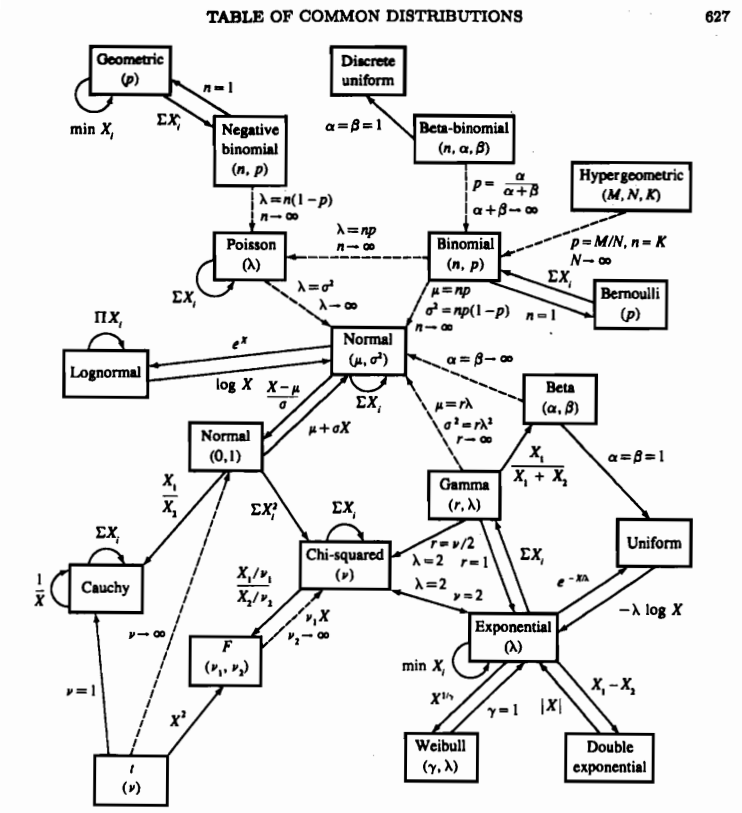
\includegraphics[width=0.36\textwidth]{Dist_fig} 

\end{figure}

% \begin{thmbox}
%\begin{thm}
\end{multicols*}
\end{document}

